\documentclass[]{agujournal2019}\usepackage[]{graphicx}\usepackage[]{xcolor}
% maxwidth is the original width if it is less than linewidth
% otherwise use linewidth (to make sure the graphics do not exceed the margin)
\makeatletter
\def\maxwidth{ %
  \ifdim\Gin@nat@width>\linewidth
    \linewidth
  \else
    \Gin@nat@width
  \fi
}
\makeatother

\definecolor{fgcolor}{rgb}{0.345, 0.345, 0.345}
\newcommand{\hlnum}[1]{\textcolor[rgb]{0.686,0.059,0.569}{#1}}%
\newcommand{\hlstr}[1]{\textcolor[rgb]{0.192,0.494,0.8}{#1}}%
\newcommand{\hlcom}[1]{\textcolor[rgb]{0.678,0.584,0.686}{\textit{#1}}}%
\newcommand{\hlopt}[1]{\textcolor[rgb]{0,0,0}{#1}}%
\newcommand{\hlstd}[1]{\textcolor[rgb]{0.345,0.345,0.345}{#1}}%
\newcommand{\hlkwa}[1]{\textcolor[rgb]{0.161,0.373,0.58}{\textbf{#1}}}%
\newcommand{\hlkwb}[1]{\textcolor[rgb]{0.69,0.353,0.396}{#1}}%
\newcommand{\hlkwc}[1]{\textcolor[rgb]{0.333,0.667,0.333}{#1}}%
\newcommand{\hlkwd}[1]{\textcolor[rgb]{0.737,0.353,0.396}{\textbf{#1}}}%
\let\hlipl\hlkwb

\usepackage{framed}
\makeatletter
\newenvironment{kframe}{%
 \def\at@end@of@kframe{}%
 \ifinner\ifhmode%
  \def\at@end@of@kframe{\end{minipage}}%
  \begin{minipage}{\columnwidth}%
 \fi\fi%
 \def\FrameCommand##1{\hskip\@totalleftmargin \hskip-\fboxsep
 \colorbox{shadecolor}{##1}\hskip-\fboxsep
     % There is no \\@totalrightmargin, so:
     \hskip-\linewidth \hskip-\@totalleftmargin \hskip\columnwidth}%
 \MakeFramed {\advance\hsize-\width
   \@totalleftmargin\z@ \linewidth\hsize
   \@setminipage}}%
 {\par\unskip\endMakeFramed%
 \at@end@of@kframe}
\makeatother

\definecolor{shadecolor}{rgb}{.97, .97, .97}
\definecolor{messagecolor}{rgb}{0, 0, 0}
\definecolor{warningcolor}{rgb}{1, 0, 1}
\definecolor{errorcolor}{rgb}{1, 0, 0}
\newenvironment{knitrout}{}{} % an empty environment to be redefined in TeX

\usepackage{alltt}

\usepackage{url} %this package should fix any errors with URLs in refs.
\usepackage{lineno}
\usepackage[inline]{trackchanges} %for better track changes. finalnew option will compile document with changes incorporated.
\usepackage{soul}
\linenumbers



% LTeX: language=en-US

\usepackage{color}
\newcommand*{\todo}[1]{\textbf{\textcolor{red}{(#1)}}}
\newcommand*{\mref}{\todo{ref}}

\usepackage{xr}
\externaldocument[SM-]{../supporting info/supp_info_hail}

% Goes against template but looks a lot nicer.
\justifying 

% Maximum 12 PUs where 1 PU = 500 words or 1 display element (figure or table).
% E.g. 

% To mark revisions:
%
%  \note[editor]{The note}
%  \annote[editor]{Text to annotate}{The note}
%  \add[editor]{Text to add}
%  \remove[editor]{Text to remove}
%  \change[editor]{Text to remove}{Text to add}

\draftfalse
\journalname{Geophysical Research Letters}
\IfFileExists{upquote.sty}{\usepackage{upquote}}{}
\begin{document}

\title{Changes in damaging hail in major Australian cities with global warming}

\authors{Timothy H. Raupach\affil{1,2,3}, Joanna Aldridge\affil{4,5}}

\affiliation{1}{UNSW Institute for Climate Risk and Response, 
                UNSW Sydney, New South Wales, Australia}
\affiliation{2}{UNSW Climate Change Research Centre, 
                UNSW Sydney, New South Wales,  Australia}
\affiliation{3}{ARC Centre of Excellence for Climate Extremes, 
                Sydney, New South Wales,  Australia}
\affiliation{4}{School of Geosciences, University of Sydney, 
                Sydney, New South Wales,  Australia}
\affiliation{5}{QBE Australia, Sydney, 
                New South Wales, Australia}

\correspondingauthor{Timothy H. Raupach}{timothy.h.raupach@gmail.com}

\begin{keypoints}
\item Hail causes more damage when hailstones are larger or coincident winds are
stronger, yet there is high uncertainty in the changes in these factors with
global warming.
\item Convection-permitting downscaled simulations were used to investigate
possible future changes in hail size and coincident wind strength over major
Australian cities and the remote Western Australian Goldfields region. \todo{JA:
state scenario and timeframe}
\item The projections indicate increases in hailstorm severity in areas around
the major population centers of Melbourne, Canberra and Sydney, with increased
windblown hail risk in the remote Goldfields region, and non-significant changes
in other studied domains. \todo{JA: confusing, doesn't say same thing as abstract}
\end{keypoints}

\begin{abstract} %% 150 words
      In Australia, hailstorms are a leading cause of insured losses, with
      damage exacerbated if hailstones are larger or there are coincident strong
      winds. Despite the high damage potential of such storms, changes to their
      frequency and severity under global warming are not well understood. Here,
      we use downscaled simulations over major cities and a remote region in
      Australia to project changes in hail frequency, hailstone size, and
      coincident wind speeds under a future scenario with
      $\sim$2.8~$^{\circ{}}$~Celsius warming over pre-industrial global mean
      temperature. The study regions cover over 60\% of the total Australian
      population. Generalized extreme value analysis was used to examine changes
      in daily maximum hail sizes and coincident wind speeds. The projections
      show higher future hail damage potential in some regions, with increases
      in hail frequency in the Sydney/Canberra and Brisbane regions, and robust
      increases in maximum hail size and coincident wind strength in the
      Melbourne and Sydney/Canberra regions.
\end{abstract}

\section*{Plain Language Summary}

Hailstorms endanger lives and damage property, leading to large insurance losses
in Australia. Hailstorms are more damaging if the hailstones they produce are
larger. They are also more damaging if there is high wind at the same time,
because the wind can push hailstones sideways into breakable materials such as
windows or house facades. We expect climate change to affect hailstorms, but
there have been few studies on how hailstorm frequency and severity may change
in future in Australia. In this study we used simulations of weather in a
future, warmer climate scenario to look at possible changes in hailstone size
and in the strength of winds when hail occurs, over major cities and a remote
area in Australia. The simulations project an increase in hail severity for the
heavily populated Melbourne and Sydney/Canberra regions, an increase in hail
frequency in Sydney/Canberra and Brisbane regions, and no significant changes in
the other areas we studied.

\section{Introduction}

Hailstorms are most damaging when the hailstones they produce are larger
\cite{Brimelow_WF_2002, Eccel_IJC_2012}, and when there are coincident strong
winds that push  hailstones laterally \cite{Changnon_JAMC_1967,
Towery_JAMC_1976}. While anthropogenic climate change is expected to affect
severe convective storms \cite{Allen_2018} and their associated hazards of hail
\cite{Raupach_NREE_2021} and extreme winds \cite{Brown_JGRA_2021}, there remains
high uncertainty and geographical heterogeneity in projections of how these
changes may manifest \cite{Raupach_NREE_2021, Brown_JGRA_2021}, and changes in
the coincidence of hail and high winds have been virtually unstudied. Here, we
use high-resolution downscaled simulations of a future, warmer environment to
compare changes in hail damage potential over hail-prone areas of Australia.
\todo{JA: suggest a bit more about the study aims/framework as this is useful
for the reader to understand upfront – ie one climate scenario, one time frame,
CMIP6 ensemble}

\todo{Impacts in Australia} Severe convective storms are responsible for insured
losses of over \$A40b in Australia from 1967 to 2023 (in 2022 dollars),
accounting for 25\% of insured catastrophe losses \cite{ICA_2024}. The largest
insured loss for any catastrophe event in Australian history, at \$A8.845b
\cite<normalized to 2022 dollars, >{ICA_2024}, was caused by the April 1999
hailstorm impacting the eastern suburbs of Sydney. Canberra and Brisbane have
also experienced hail events with normalized losses over \$A1b \cite{ICA_2024}
\todo{check ref}. 

\todo{Reasons for combining hail and wind} Hail and convective winds are often
studied separately, with typical severe convective storm catastrophe models
generating synthetic event sets of hail and wind hazards as separate event
footprints \mref{}. However, the coincidence of wind and hail is an important
driver of loss. Wind-driven hail, both due to its greater force and oblique
angle of impact, has greater potential to injure people, destroy crops
\cite{Changnon_JAMC_1967, Towery_JAMC_1976} and cause damage to the built
environment, such as damaging cladding to external walls, breaking windows of
buildings and motor vehicles and letting rainwater inside to damage internal
fixtures and contents \mref{}. Examination of recent high-loss hail events in
Australia shows that wind is often mentioned as a contributing factor \mref{}.
Common thresholds for damaging conditions include hail over 2 cm in diameter
\mref{} or wind gusts over 90 km h$^{-1}$ \cite{Allen_2018}. Wind driven hail
events are defined here as hail exceeding 5 cm in diameter  and wind gusts
exceeding 100 km/h (27.8 m/s) occurring in the same system within a one-hour
timeframe \mref{}. Wind driven hail events are most likely to be associated with
supercells where downbursts occur \mref{}. Observational data in the United
States of America (USA) identified squall lines, isolated cells, and clusters of
cells as the most frequent systems associated with wind driven hail
\cite{Carletta_2010}. \cite{Bell_WF_2023} compiled 1646 hail and wind damage
swaths for the mid-west of the USA using satellite observations for use in
future understanding of the frequency of these events. No such studies for
Australia have been identified.

\todo{What is known of hail and wind changes with global warming}
\cite{Allen_JC_2014} used an environment-based approach to suggest an increase
in severe thunderstorm incidence in south-east Australia, although with a wide
range of uncertainty. \cite{Walsh_CC_2016} review the current and future
storm-related wind and hail hazard in Australia and found future projections of
wind hazard increase along the populated east coast of Australia. \todo{More to
add here. JA: You need to add your own studies – I suggest we could move this to
be Para 2 in the introduction?}

\todo{JA's text re case study events} A selection of recent large loss causing hail events in Australia associated with both giant hail and strong winds include:

\begin{itemize}
\item October 2020 ``Hailoween'' hail storm impacting the southern suburbs of
Brisbane;
\item January 2020 ``Tri City'' hail storm impacting Canberra, Melbourne and
Sydney;
\item April 2020 Rockhampton hail storm impacting the Queensland towns of
Rockhampton and Yeppoon.
\end{itemize}

These three case studies are described in more detail below.

\todo{JA: To Add: Coloured charts? I don’t have any that aren’t proprietary. JA
provided black and white synoptic charts in word document.}

\todo{Hailoween} The October 2020 ‘Hailoween’ hail storm generated a series of
at least nine super cells in a corridor from Amberley to Logan that generated
giant hail stones reported as 7 cm in Gympie, giant hail up to 14 cm at
Forestdale, 13cm at Hillcrest, 9.5 cm at Amberley, 8 cm at Springfield, 7 cm at
Gatton, and 5 cm at Seventeen Mile Rocks. The hardest hit suburbs were
Singfield, Springfield Lakes, Rosewood, Thagoona and Willowbank. Strong winds
were also recorded, with 100 kmh 3-second gusts occurring around Moreton Bay and
wind damage evident from Redcliffe to Kingston. The State Emergency Service
received 2900 call outs and power outages affected 95 000 people. The storms
were associated with a series of complex fronts and embedded lows in the monsoon
inland trough, following a week of instability over eastern Australia (Figure
X). The Queensland Reconstruction Authority (QRA)’s initial assessment
immediately after the hailstorm identified 520 properties with severe damage,
602 dwellings with moderate damage and 652 properties with minor damage.
Extensive damage was reported to roofs, skylights, solar panels, interior,
awnings, windows, shutters, ceiling collapse, falling trees. Water ingress
following hail damage was widespread, leading to damage to interior walls and
floors, mould, and contents damage. Some houses experienced hail damage through
the roofs, solar panels and interior ceiling into the living areas of the home.
This event resulted in an insured loss of \$A1.056b from around  44,700 claims
\todo{(Insurance Council of Australia, 2024)}. \todo{Reference:
https://knowledge.aidr.org.au/resources/hailstorm-south-east-queensland-2020/}

\todo{Tri-city storm} The 20th January 2020 ``Tri-City'' storms impacted a wide
area of eastern Australia immediately following the devastating ``Black Summer''
bushfires. The storms impacted three major cities: Canberra, Sydney and
Melbourne as well as country NSW areas of Queanbeyan and Goulburn. Canberra
received 5–7 cm hail impacting the Central Business District and densely
populated inner suburbs including the Australian National University. A 117 km h
wind gust was recorded at Canberra Airport. Melbourne received hail of up to 5.5
cm over the southeastern suburbs along with damaging winds, heavy rainfall and
flash flooding. Sydney received up to 7 cm hail over the outer southern suburbs
of Campbelltown and the Sutherland Shire. The meteorological situation showed an
inland trough extending from central Queensland through southeastern Australia,
with an upper level low and associated surface level low creating moist unstable
air. The extensive damage in Canberra included broken windows and sky lights in
homes and commercial buildings, flooding, and thousands of cars damaged by
hailstones.  Wind damage includes fallen trees, branches and power lines, and
blocked roads. There was structural damage to buildings at the Australian
National University and civil buildings in the central business district. This
event resulted in around 132 000 claims and a \$A1.68b insured loss
\todo{(Insurance Council of Australia, 2024)}. \todo{Reference:
\url{https://knowledge.aidr.org.au/resources/hailstorms-and-heavy-rainfall-victoria-january-2020/}}

\todo{Rockhampton} The April 2020 hailstorm impacted the central Queensland
towns of Rockhampton and Yeppoon and surrounding areas located on the Tropic of
Capricorn. The weather pattern was due to an upper-level trough crossing central
Queensland combined with a surface trough. Storm activity propagated from inland
moving northeast to the coast, with a large supercell impacting the corridor
from Rockhampton to Yeppoon. Giant hail of 8 to 12 cm was reported as well as
100 kmh 3-second wind gusts. Damage included holes in roofs, smashed windows and
car windscreens, some flooding and tree damage. The timing of this event during
the first Covid lockdown complicated recovery efforts. An insured loss of
\$A503m from around 15 000 claims was incurred (Insurance Council of Australia,
2024). In the Whitsunday region, golf ball size hail was reported in Sarina. The
time of year, size of hail and the tropical latitude of this event made it
highly unusual. \todo{References:
\url{https://www.swissre.com/australia_newzealand/insights/rockhampton--hail.html}
\url{https://www.earlywarningnetwork.com.au/news/record-hailstorms-lash-central-queensland}
\url{https://www.abc.net.au/news/2020-04-20/supercell-storm-causes-widespread-damage-in-central-queensland/12163780}}

\todo{Australian context re building codes} While wind loadings are currently
considered in the Australian building code \cite{ABCB_2024} under standard
AS1170.2 \cite{Standards_2021}, the impact of hail and wind-driven hail is not
currently considered in Australian building design. The \citeA{ACSE_2022}
discuss hail loading on roofs and acknowledge that this effect is not accounted
for under the current design standards. The April 2015 hail event impacting
western Sydney is discussed including the collapse of warehouse buildings from
hail loading on roofs. A guide of ultimate limit and service limit state designs
for various building types is presented, but wind driven hail is not considered.
Some roofing products are tested for hail impacts against standards, but many
products are unrated. In the ICC building code \cite{ICC_2008}, hail is
considered in two hail regions in the USA defined using observational data:
moderate and severe, depending on the likelihood of at least one day of 1.5--3
mm \todo{check} hail in a 20-year period. This code requires testing of roofing
materials such as asphalt, wood and slate shingle, clay or concrete tiles, metal
roofing panels and shingles in these zones. The changing occurrence of hail over
time is not considered in that code. In Canada, while hail impact is not
considered in the current building code,  change is being sought in the
aftermath of the 2020 Calgary hailstorm which caused \$C1.4b of insured loss.
Resilience measures may include increasing roof slope, using resistant roofing
materials and roof underlays \cite{ICLR_2018}. A finding was that a steeper roof
limits damage from wind-driven hail on the leeward side of a property. The lack
of research into impact resistant non-roof housing elements, such as windows,
doors, sidings, fascia and skylights, is noted, and these elements are often
subject to damage in the most destructive storms.

\todo{What we have done here} Here, we seek to understand how the coincidence of
extreme winds and damaging hail may change in a future climate in Australia. We
conducted analyses covering the major Australian cities of Perth, Adelaide,
Melbourne, Canberra, Sydney, and Brisbane, and a remote region around the town
of Kalgoorlie in the Western Australian Goldfields. The populations of these
cities covers over 60\% of the total Australian population \mref{}. Proxy-based
climatologies show these regions to be hail-prone \cite{Raupach_npjCAS_2023}.

\todo{JA: mention additional results that are presented in the results section
and why we ar e considering these ie regional correlations in hail trends,
changes in convective parameters. ``We investigate regional correlations in hail
trends both directly from the hail size datasets and indirectly via the trends
in convective parameters, in order to better understand the potential for growth
in hail hazard in the domains surrounding Australia’s major population centres.
Growing risk in multiple locations may present a challenge to community
resilience and the insurance industry by requiring more robustness and
redundancy in both the supply chain and capital to repair damage across several
states. Understanding the trends in the contributing convective parameters aids
our understanding of the driving processes behind projected hail changes.''}

\section{Methods}

\subsection{Simulations of historical and projected weather}

Historical and future simulations were produced using the Advanced Research
Weather Research and Forecasting (AR-WRF) weather model version 4.4.1
\cite{Skamarock_2021} for six nested domains. Two model configurations were
used, with settings other than the domain configurations the same for both
(Supporting Information Table \ref{SM-tab:schemes}). In total, we used two
coarse- ($\sim$27 km grid spacing), four medium- ($\sim$9 km), and six
fine-resolution ($\sim$3 km) domains with a parent-child scaling ratio of three
(Supporting Information Figure \ref{SM-fig:domains}). WRF-HAILCAST
\cite{Adams-Selin_WF_2019} was enabled for the fine-resolution domains, to
estimate maximum hailstone diameters at the surface. Boundary condition inputs
were prepared using the \texttt{nc2wrf} code of \citeA{Xu_code_data_2021}. 

Simulations were run for two epochs of 20 convective seasons each: the
historical epoch ran from 1989 to 2009, and the future epoch from 2080 to 2100.
For each convective season, simulations were run from 00Z September 30 to 18Z
February 28, with hourly output resolution. Outputs were converted to local
summer time and subset to cover October 1 to February 28 inclusive in each
season. For each season the 14 to 16 simulated hours on 30 September local time
were discarded as model spin-up time. Model outputs provide instantaneous hourly
values for most variables, including wind speed at 10 m \todo{JA: above ground
level?}. In contrast, for each grid point and each hour, HAILCAST output the
maximum hail diameter over all model time steps during the previous hour. The
time step for the coarse domain was set to 100 s, but reduced to 80 s or 60 s
for simulation days on which Courant-Friedrichs-Lewy (CFL) errors occurred.
HAILCAST was run at every model time step, so on those days for which the time
step was reduced, HAILCAST ran more often. However, here we use maximum hail
sizes per day, and the sample of hail sizes per day is large, so we expect
minimal effect of this time step variability. Except for the overall maxima
shown in Section \ref{sec:overall_maxima}, we subset all our analyses to
consider only times and locations where there was non-zero surface hail recorded
in the preceding hour. Wind speeds and convective parameters are thus
instantaneous values in temporal proximity to hail occurrences.

\subsection{Processing of simulation outputs}

Examination of maximum hail size fields showed that HAILCAST occasionally
produced unreasonably large hail sizes, particularly over water bodies
(Supporting Information Figure \ref{SM-fig:maxes_with_removed_pts}). Since our
focus is on hail hazard on land, we subset the data to land areas using the WRF
land mask with small holes filled and a slight erosion applied so that points
over the ocean, large bodies of water, or directly over the coastal boundary are
not considered in this study. Further, we removed from consideration any
HAILCAST value of surface hail over 180 mm diameter \cite<this value being
greater than the largest hail ever observed in Australia, at $\sim$16
cm,>{BOM_2021} \todo{JA: discarding HAILCAST outputs >18 cm – would it be more
reasonable to cap it then discard this data?}. HAILCAST has been updated in more
recent versions of WRF than used here, and while the updated version reduces the
occurrence of unrealistically large hail sizes the changes do not affect the
majority of HAILCAST results, meaning that removing very large hail sizes, as we
do here, leaves a reasonable dataset for analysis (pers. comm. B. Adams-Selin,
2024). In all, less than 0.006\% of non-zero hail-diameter values (not over
water) were removed for being too large, per domain. Convective parameters were
calculated as described in \citeA{Raupach_MWR_2023}. \todo{JA: Suggest
mentioning what the parameters are and maybe a brief description.}

\subsection{Statistical modelling of extreme values}

Extreme value analysis was completed using the R \cite{R_software} package
\texttt{extRemes} \cite{Gilleland_JSS_2016}. Block maxima were defined as daily
maximum hailstone sizes and wind speeds at hail locations per domain, under the
assumption that such time series can be considered independent \cite{Coles_2001}
because single hail storms do not last more than one day. Generalized extreme
value (GEV) distributions were fitted to each series of block maxima. We used
quantile-quantile (QQ) plots \cite{Coles_2001} and the Kolmogorov–Smirnoff (KS)
test to assess the goodness of fit of the GEV distributions, by examining the
similarity of the empirical distributions of block maxima and values drawn from
the fitted GEV distributions. The KS test was also used to examine the
(dis)similarity of GEV distributions fitted to historical versus future epochs.
When the KS test was used, we generated a probabilistic view of the similarity
between distributions by drawing 1000 values from the GEV distribution(s),
applying the KS test, and repeating this process 100 times to generate 100 KS
test results. \todo{JA: suggest moving the EV section below the Data Section.}

\section{Data}

Boundary conditions used for the simulations were bias-corrected data for
downscaling by \citeA{Xu_SD_2021}. These boundary conditions have a mean climate
and interannual variance derived from European Centre for Medium-Range Weather
Forecasts Reanalysis 5 \cite<ERA5,>{Hersbach_QJRMS_2020}, with a non-linear
trend derived from the ensemble mean of 18 Coupled Model Intercomparison Project
Phase 6 \cite<CMIP6,>{Eyring_GMD_2016} models \cite{Xu_SD_2021}. Future
projections used the ``middle-of-the-road'' SSP2-4.5 shared socioeconomic
pathway \cite<SSP,>{ONeill_GEC_2017}. On average the historical period in our
simulations (1989--2019) had a global mean temperature 0.39 K above
pre-industrial temperatures \cite<1850--1990, using the CMIP6 35-model
ensemble,>{Gutierrez_2021} while the future period (2080--2099) had a global
mean temperature 2.81 K over pre-industrial temperatures. The historical and
future epochs were thus separated by 2.42 K of warming.

\section{Results}
\label{sec:results}

\subsection{Overall maxima}
\label{sec:overall_maxima}

Before taking a more rigorous statistical approach, it is useful to consider the
maps of overall maxima for the quantities of interest here: hailstone size, and
10 m wind speed at hail hours. Figure \ref{fig:max_hail_sizes_by_domain} shows
overall maximum hail sizes across each domain for each epoch. Hailstorm tracks
are visible. By eye, an increase in maximum hail sizes is apparent for domains
other than Perth and Brisbane, with increases in storm coverage or activity in
the Adelaide, Goldfields (Kalgoorlie), Melbourne and Canberra/Sydney domains.
Maximum wind speeds at hail hours are more widespread in the future scenarios
than the historic scenarios, with an eastward expansion in areas experiencing
maximum wind speeds in the Brisbane and Adelaide domains and a southern shift in
the Goldfields (Kalgoorlie) region (Supporting Information Figure
\ref{SM-fig:max_wind_by_domain}).

\begin{figure}[!h]
      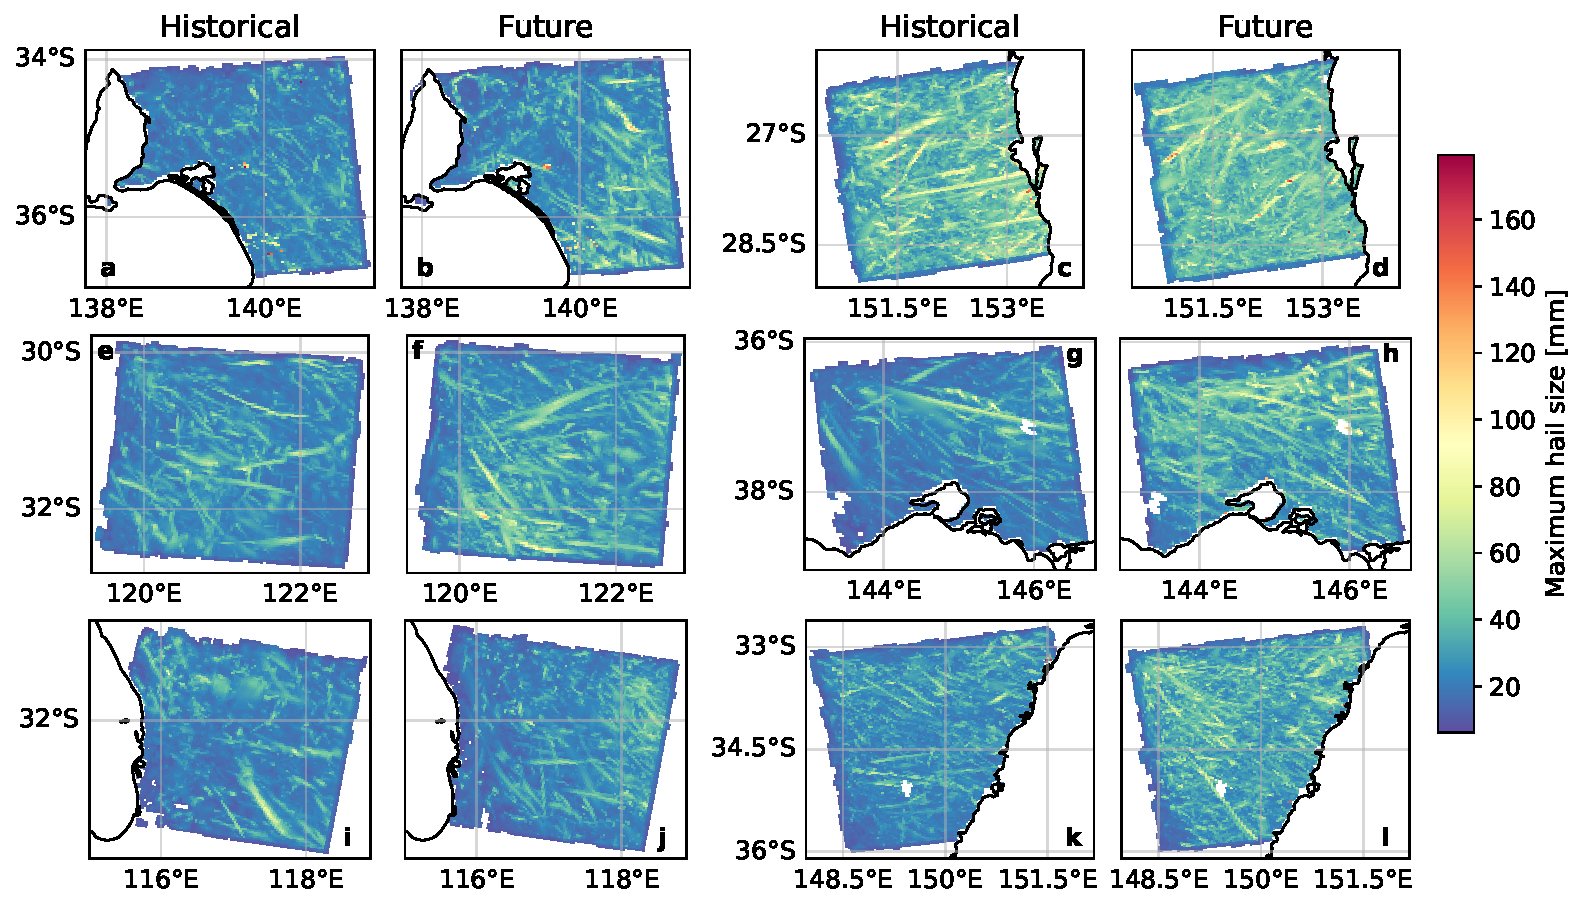
\includegraphics[width=\textwidth]{figures/max_hail_sizes_by_domain}
      \caption{Maximum hail sizes in historical and future climates, for
      Adelaide (a, b), Brisbane (c, d), Goldfields (Kalgoorlie) (e, f),
      Melbourne (g, h), Perth (i, j) and Sydney/Canberra (k, l) domains.
      \todo{JA: the time period in past and future maps is not equal? 30 years
      vs 20 years?} \todo{JA: – (k,l) can you plot the location of Canberra and
      Sydney? I feel the reviewers might comment that this domain has a boundary
      issue coming from the upper left corner. I don’t feel that hail storms
      typically propagate NW to SW in this region, they typically track from the
      W or SW? This appears to the only domain where the behaviour of the hail
      storms changes in the future, if you think that is real, then we should
      discuss it in the text as its interesting.}}
      \label{fig:max_hail_sizes_by_domain}
\end{figure}

\subsection{Changes in frequency of hail}

Table \ref{tab:frequency} shows changes in the frequency of hail days across the
six study domains. There are significant increases in hail frequency in the
Sydney/Canberra and Brisbane domains, with a 29\% increase in seasonal hail days
in the Sydney/Canberra region. There are small non-significant frequency
decreases in Adelaide, the Goldfields (Kalgoorlie) and Melbourne domains, and an
indication of an increase in seasonal hail days in the Perth region, albeit not
statistically significant. The variability in seasonal hail days is similar
between epochs.

\begin{table}[!ht]
      \centering
      \caption{Mean and standard deviation of seasonal hail days in the historic
      and future simulations, and relative future changes with 95\% confidence
      interval according to Welch's two-sample t-test, per domain. Statistical
      significance of the change calculated by Welch's two-sample t-test is
      indicated by $\ast{}$ for a 90\% confidence level ($p < 0.1$) and
      $\ast{}\!\ast{}$ for a 95\% confidence level ($p < 0.05$).}
      \label{tab:frequency}  
      \begin{tabular}{lrrr@{}l@{}r}
            \hline
            Domain & Historic days & Future days & \multicolumn{3}{r}{Future change} \\ 
            \hline
Adelaide  & 8.7 $\pm$ 4.2 & 8.35 $\pm$ 4.9 & -4\% & $$ & (-38\% to 30\%) \\Brisbane  & 32.95 $\pm$ 8.3 & 37.8 $\pm$ 8.8 & 15\% & $\,\ast{}$ & (-2\% to 31\%) \\Kalgoorlie  & 10 $\pm$ 6 & 9.8 $\pm$ 5.2 & -2\% & $$ & (-38\% to 34\%) \\Melbourne  & 11.7 $\pm$ 5.9 & 11.5 $\pm$ 7.1 & -2\% & $$ & (-37\% to 34\%) \\Perth  & 6.8 $\pm$ 4.9 & 7.55 $\pm$ 4.9 & 11\% & $$ & (-35\% to 57\%) \\Sydney/Canberra  & 24.3 $\pm$ 9.4 & 31.4 $\pm$ 9 & 29\% & $\,\ast{}\!\ast{}$ & (5\% to 53\%) \\
            \hline 
       \end{tabular}
\end{table}

\subsection{Extreme value analysis}

\todo{JA: For Sydney and Melbourne domains (or all of them) you need to plot the
 extreme value curves to show how the 3 parameters are changing the shape of the
 curves. I see the curves currently are presented after the change in the
 parameters. Would it be better to start with these curves rather than the
 change in the parameters?}

\todo{JA: A reviewer might ask if these results are sensitive to threshold. You
could also chose to keep the 3rd parameter constant if it is physically
reasonable that the whole shape of the tail of the curve would not change (we
force this for cyclone and flood, we do not expect the curve to increase forever
with increasing RP due to physical constraints).}

\subsubsection{GEV goodness of fit}

GEV models were fitted to time series of daily maximum hail sizes and 10 m wind
speeds at hail hours (Supporting Information Figures
\ref{SM-fig:timeseries_hail} and \ref{SM-fig:timeseries_wind}). QQ plots for
hail size show acceptable agreement with some model overestimation of high
quantiles (Supporting Information Figure \ref{SM-fig:qq_hail}), while QQ plots
for wind speed at hail hours show excellent agreement between modelled and
empirical quantiles (Supporting Information Figure \ref{SM-fig:qq_wind}). In all
cases where the model was compared to empirical values, either all or the bulk
of KS test $p$ values were above the 0.05 level, indicating that the null
hypothesis that the two samples are drawn from the same distribution can not be
rejected (Supporting Material Figure \ref{SM-fig:ks_pvals}). The QQ plot and KS
test results show that the GEV models have sufficient goodness of fit for the
analyses here. 

\subsubsection{Significance of changes}

Having determined that the GEV fits to empirical data are valid, we now consider
whether the fitted models show any significant difference between the historical
and future epochs. Figure \ref{fig:gev_parameters} shows the fitted parameters
and their confidence intervals for all the GEV models used in this study. The
models fitted for the Melbourne and Sydney/Canberra domains both show
significant differences between epochs in the location or scale parameters for
both hail size and wind at hail hours, whereas the models for the other domains
have parameters with overlapping confidence intervals. These results are further
supported by the $p$ value distributions from KS tests when historical models
are compared to future models (Supporting Information Figure
\ref{SM-fig:ks_pvals}). The null hypothesis that the samples are drawn from the
same distribution can be rejected for the Melbourne and Sydney/Canberra domains
for both maximum hail size and maximum wind speed at hail hours, and for the
Perth domain for wind only. To be conservative, we conclude that the changes in
maxima between epochs are significant in the Melbourne and Sydney/Canberra
domains, but not significant in the other domains.

\begin{figure}[!ht]
      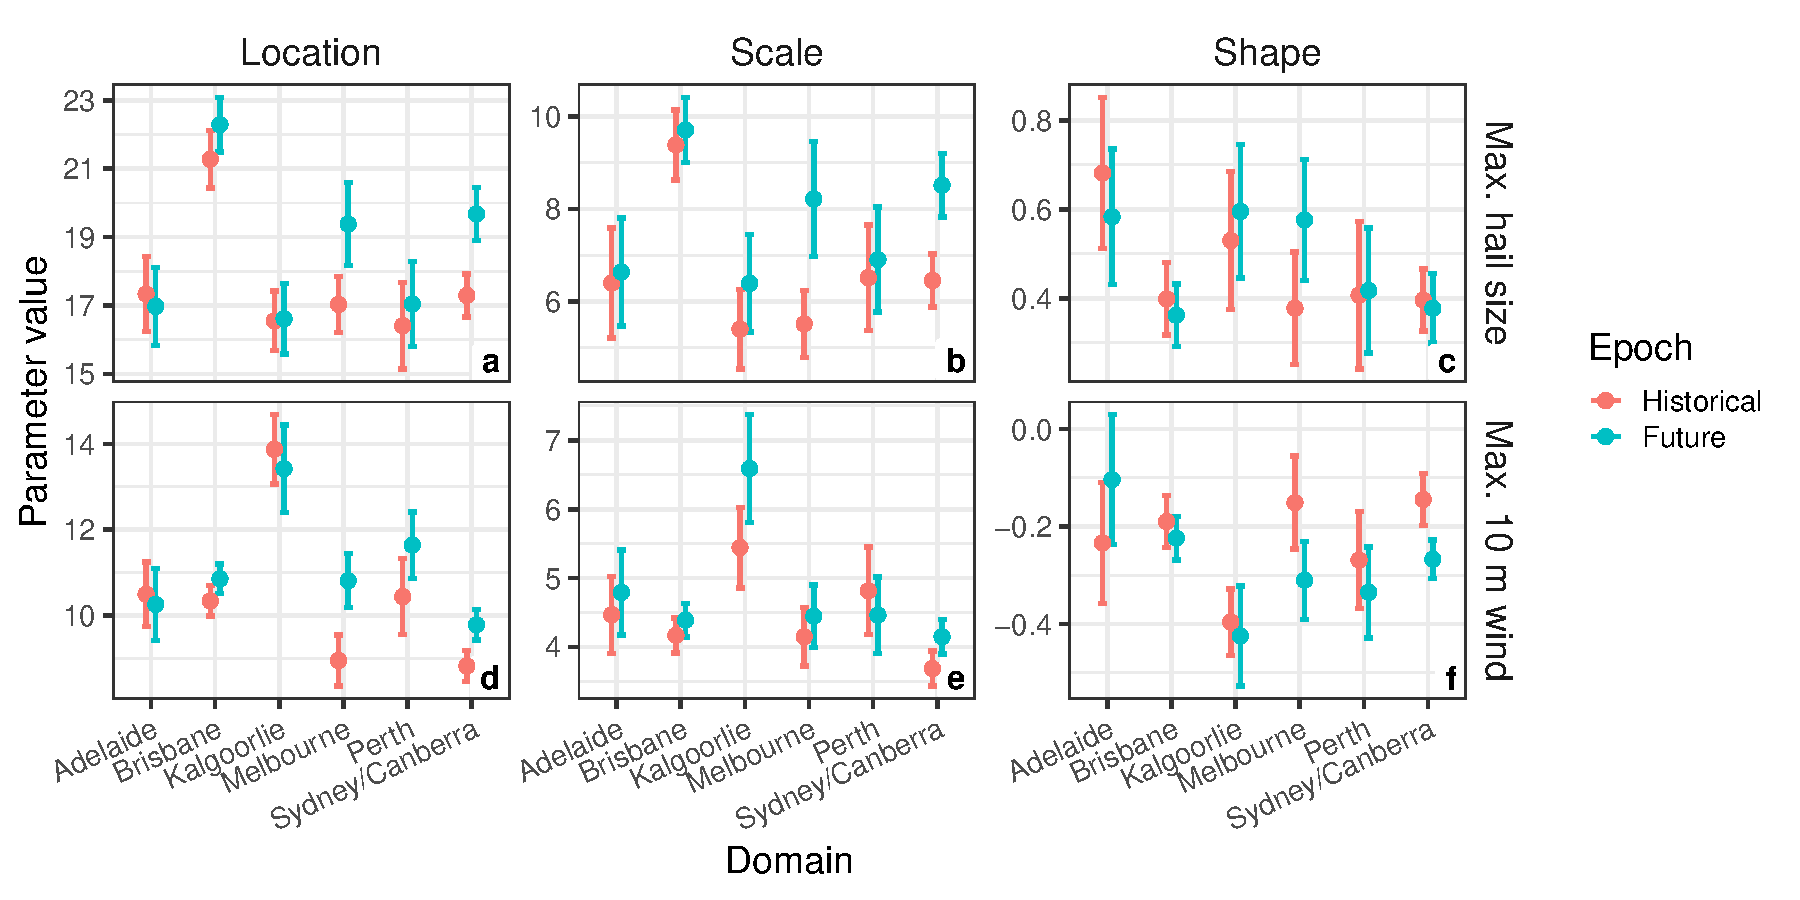
\includegraphics[width=\textwidth]{figures/fit_params}
      \caption{Location (a, d), scale (b, e), and shape (c, f) parameters for
      fitted GEV distributions for maximum hail size (a--c) and 10 m wind at
      hail hours (d--f). Parameter values are shown as a point and whiskers show
      95\% confidence intervals.}
      \label{fig:gev_parameters}
\end{figure}

\subsubsection{Return periods}

\todo{JA: should be showing the return period of hail days in years}
\todo{JA: Extension – can this be expanded into bivariate GEV bt wind and hail?}

Figure \ref{fig:return_periods_probs_hail} shows return period curves for
maximum hail size and maximum wind speed at hail hours. Because our analysis is
limited to hail days, the return periods are in number of hail days, not overall
days. It is not uncommon for return period models based on the GEV family to
produce non-physical extreme values such as the extremely large hail sizes
predicted for large return periods here \cite[p. 66]{Coles_2001}. We take the
advice of \citeA{Coles_2001} and interpret the results here based on the shorter
return periods, thus keeping physical principles in mind. In Melbourne and
Sydney/Canberra, the two domains with significant changes, there are increases
in the maximum expected hail size for return periods longer than about three
hail days, with the largest increase in the Melbourne region where the return
period for 100 mm hail is reduced from more than 100 hail days to about 30 hail
days. In both domains with significant changes the return period for lighter
winds (less than about 18 m s$^{-1}$) is markedly shorter in the future
scenario, but the return period for very strong winds is longer in the warmer
scenario. For the other domains, with non-significant differences in GEV
distributions, the most notable changes are a decrease in strong wind return
periods for Adelaide and Goldfields (Kalgoorlie) regions and light wind return
periods in the Perth region.

\begin{figure}[!ht]
      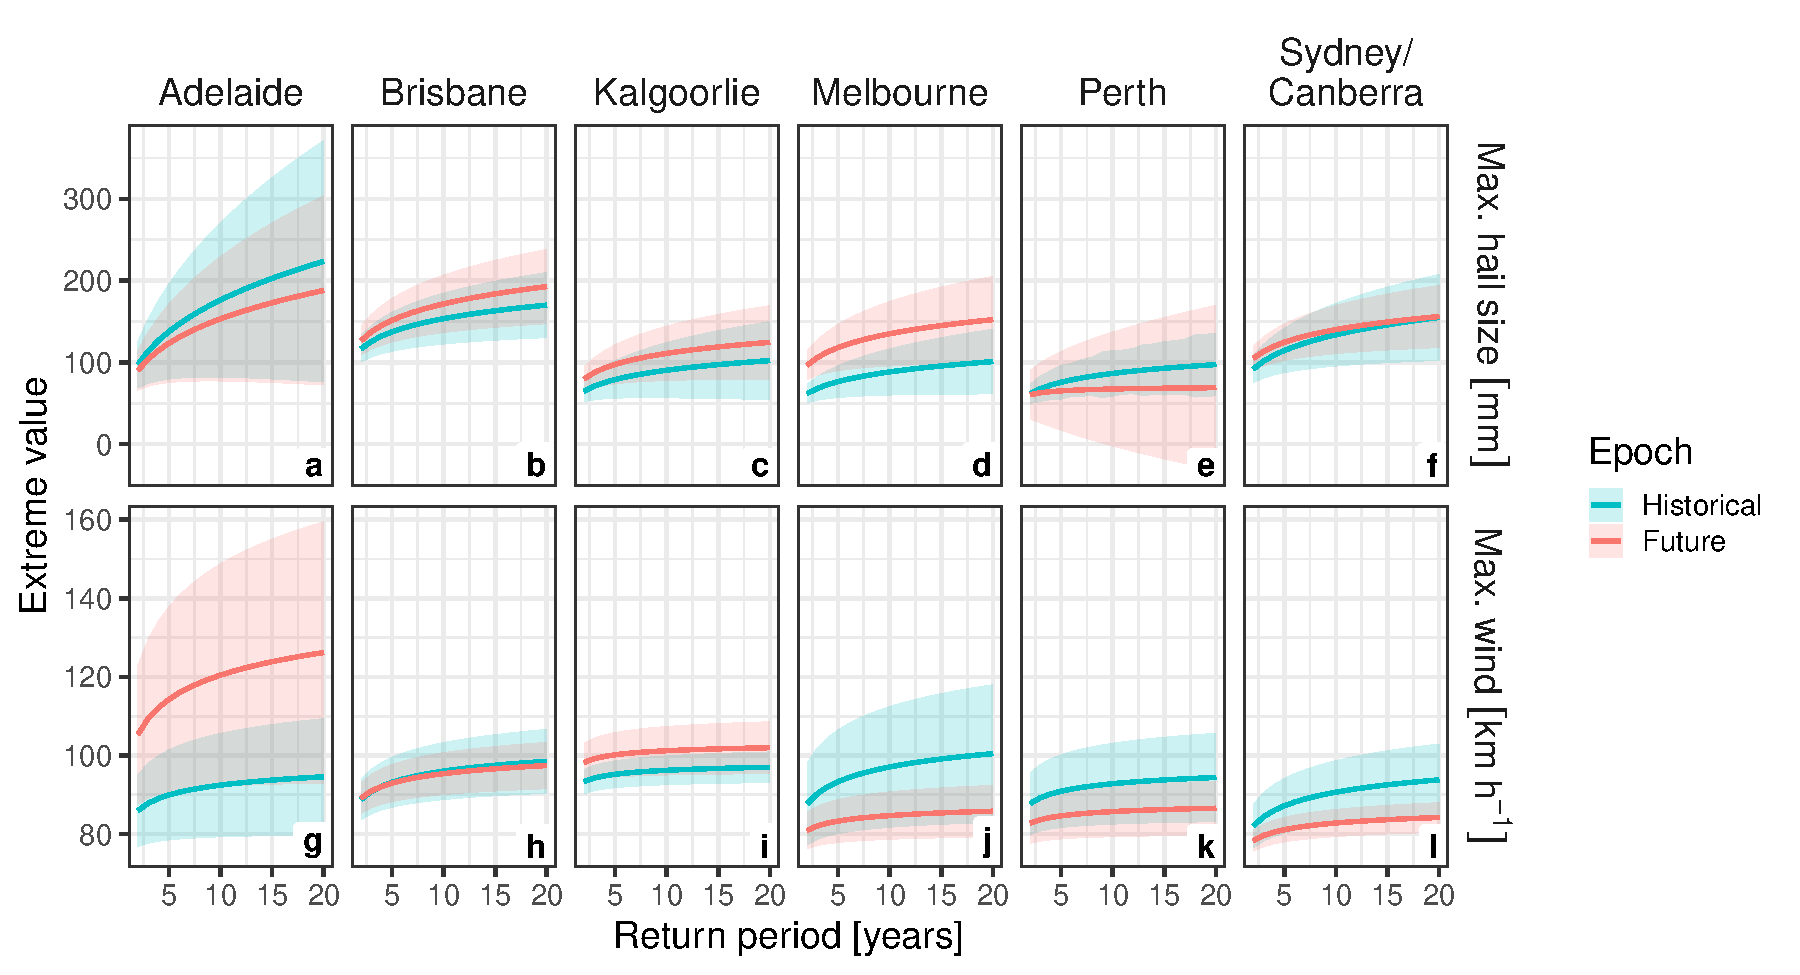
\includegraphics[width=\textwidth]{figures/return_periods}
      \caption{Return period plots for maximum hail size (a--f) and maximum wind
      at hail hours (g--l) for the domains of Adelaide (a, g), Brisbane (b, h),
      Goldfields (Kalgoorlie) (c, i), Melbourne (d, j), Perth (e, k), and
      Sydney/Canberra (f, l). \todo{JA: I find the x-axis RP unit expressed as
      hail days to be unusual – we want to measure if the number of days with
      giant hail is increasing so I think the unit has to be years Since you
      have extracted hail days in the season, then the measure of time is the
      full season.}}
      \label{fig:return_periods_probs_hail}
\end{figure}

\subsubsection{Probability of exceeding damaging thresholds}

\todo{JA: is hail threshold 2 cm or 5 cm? I suggest to keep repeating the threshold.}



Figure \ref{fig:thresholds} shows the probability of a hail day producing
various damaging hail and wind thresholds at hail hours (numerical results are
shown in Supporting Information Table \ref{SM-tab:exceedence_probs}), comparing
historical to future epochs. For hail, we examine the probability of a hail day
producing severe (20 mm), giant (50 mm), and 100 mm hail, while for wind we
examine 80 and 100 km h$^{-1}$ as damaging thresholds. In the Melbourne domain
for any given hail day, the probability of severe hail jumps from
$\sim$46\% in the historical epoch to
$\sim$61\% in the future scenario, while
giant hail probability roughly triples (from $\sim$4\% to $\sim$13\%), and 100 mm
hail is more than 5 times more likely (from $\sim$1\% to $\sim$4\%) in the
future epoch. In the Sydney/Canberra domain, any given hail day has a
probability of severe hail of $\sim$49\% in the historical epoch which increases to
$\sim$62\% in the future scenario,
while giant hail probability ($\sim$6\% to $\sim$10\%) and
100 mm hail probability ($\sim$1\% to $\sim$2\%) both
come close to doubling in the future epoch. Other non-significant increases in
severe hail probability are shown for Brisbane, Perth, and Goldfields
(Kalgoorlie) areas, with non-significant decreases in the Adelaide region, and
the Goldfields region shows a non-significant increase also for giant hail
probability. In Melbourne and Sydney/Canberra, the domains with significant
differences, the probability of damaging winds at hail hours on a hail day
decreases by about half for 80 km h$^{-1}$ wind speed at hail hours.
Non-significant changes include an increase in the probability of 80 km h$^{-1}$
wind speed at hail hours in the Goldfields (Kalgoorlie) region (from
$\sim$9\% to
$\sim$13\%) and Adelaide domain (from
$\sim$2\% to
$\sim$5\%), and for 100 km h$^{-1}$
winds at hail hours for the Adelaide region (from $\sim$0\% to $\sim$1\%).
Other than for Adelaide, the probability of hail days producing 100 km h$^{-1}$
wind speed at hail hours is close to zero in all domains across both epochs. 

\begin{figure}[!ht]
      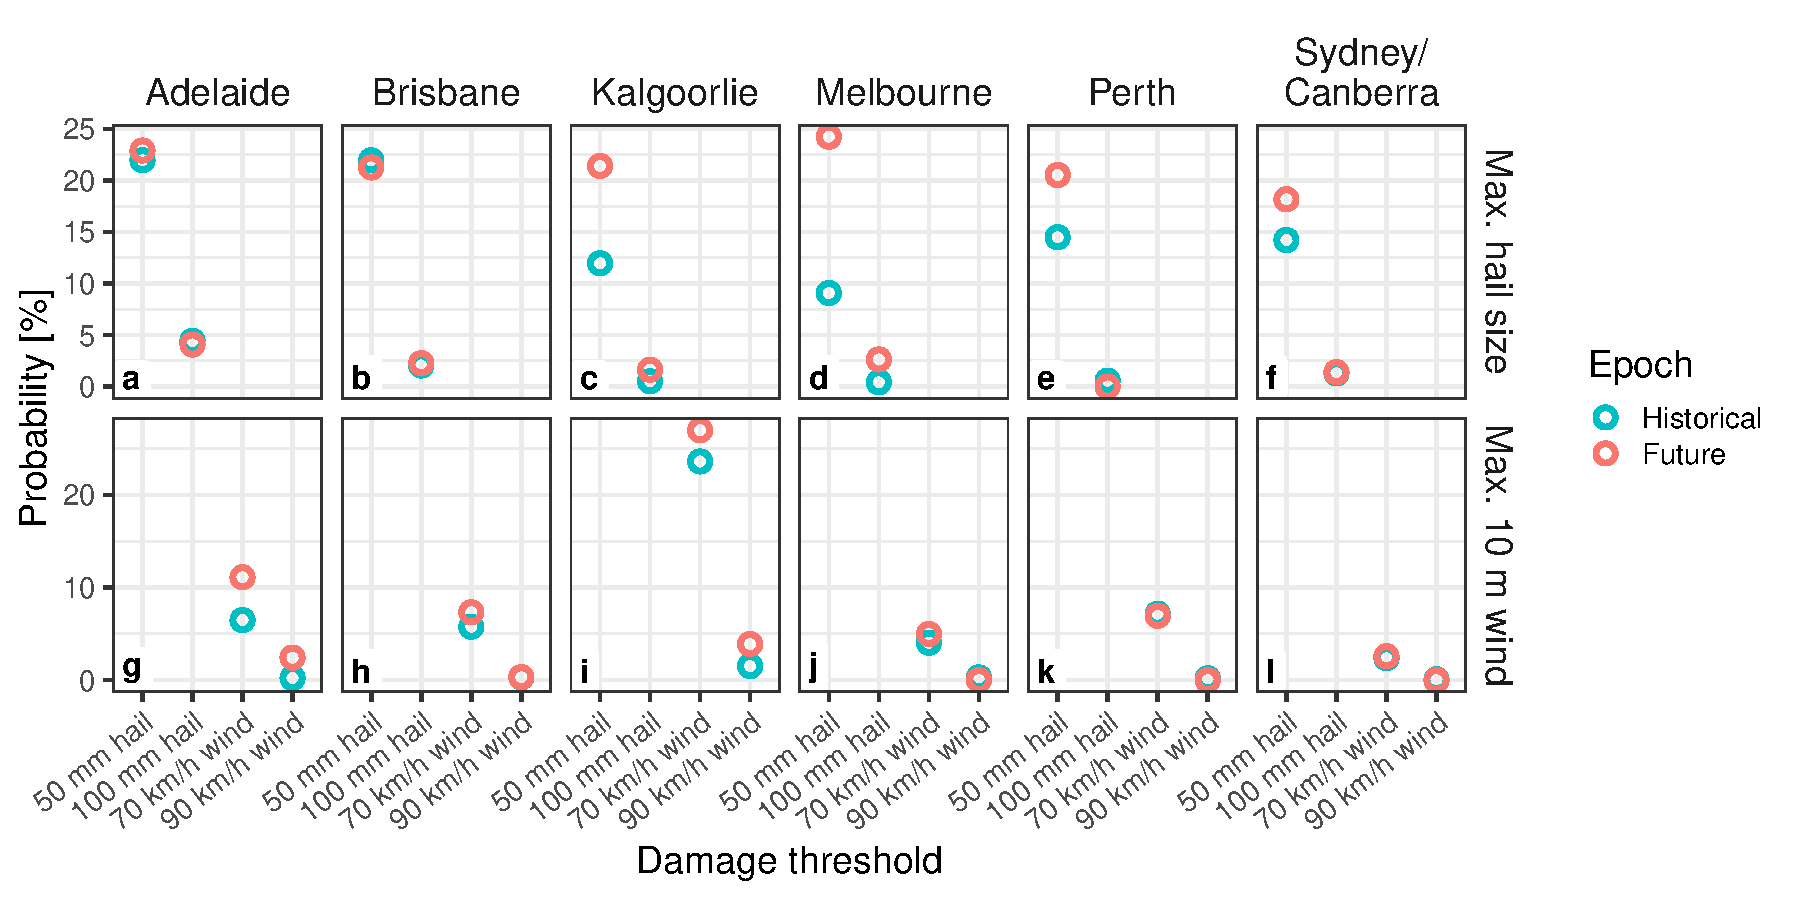
\includegraphics[width=\textwidth]{figures/threshold_probs}
      \caption{Changes in the probability of exceeding thresholds on hail size
      (a--f), and 10 m wind speed at hail hours (g--l), on any given hail day,
      for the domains of Adelaide (a, g), Brisbane (b, h), Goldfields
      (Kalgoorlie) (c, i), Melbourne (d, j), Perth (e, k), and Sydney/Canberra
      (f, l). \todo{JA: can the significant results have filled in circles?}}
      \label{fig:thresholds}
\end{figure}

\subsection{Changes in relevant atmospheric properties}

Table \ref{tab:ing_changes} shows projected changes in daily mean hail size,
wind speed, and storm-relevant atmospheric properties, at hail times, in the
future compared to historical simulations. Unlike in the extreme  value analysis
above, here we used mean values for each season and test for differences between
epochs using Welch's t-test. Mean hail size shows statistically significant
increases \todo{JA: quantify increase here} in Melbourne and Sydney/Canberra,
aligning with the extreme value analysis results for maximum hail size, but here
there is also a significant increase in the Brisbane domain. Changes in mean
wind are generally small, with the only significant changes being increases in
the Perth and Sydney/Canberra domains. Changes in wind shear are varied, with a
small significant increase in Kalgoorlie and a small significant decrease in
Brisbane. Increases of $\sim$1\% in temperature at 500 hPa, and 8-10\% in
freezing-level and melting-level heights are significant in every domain.
Atmospheric instability increases in all domains, with significant increases in
convective available potential energy (CAPE) at hail times in Adelaide,
Brisbane, Melbourne, and Sydney/Canberra regions, while the results for lifted
index (LI) are more mixed with fewer significant changes. Convective inhibition
(CIN) also became stronger in all domains with significant decreases in
Adelaide, Brisbane, the Goldfields (Kalgoorlie), Melbourne, and Sydney/Canberra.
Lapse rate changes are generally small, although significant increases are shown
in Brisbane and Sydney/Canberra. The extreme value analysis results for the
domains where they showed significant changes, Melbourne and Sydney/Canberra,
are supported by the large increases in convective instability and convective
inhibition and freezing level height, that would support storm development,
strong updrafts, and survival of large hailstones to the surface. Wind shear
changes are not significant, indicating that these changes in damage are driven
more by changes in instability than shear. In the Brisbane domain there is more
of a balance between modest yet significant increases in instability and
decreases in wind shear, indicating that in this domain there may be more
offsetting of these two environmental factors leading to no significant change
in damage potential in the GEV analyses.

\begin{table}[h!]
      \caption{Projected relative changes in mean hail size, 10 m wind (Wind),
      bulk vertical wind shear from 0-6 km (S06), convective available potential
      energy (CAPE), convective inhibition (CIN), lifted index (LI), temperature
      at 500 hPa (T500), lapse rate from 700 to 500 hPa (LR), freezing-level
      height (FLH), and melting-level height (MLH), for hail times by domain.
      Statistical significance of the difference between historical and future
      seasonal mean values, calculated using Welch's two-sample t-test, is shown
      by $\ast{}$ for the 90\% confidence level, $\ast{}\!\ast{}$ for the 95\%
      confidence level, and $\ast{}\!\ast{}\!\!\ast{}$ for the 99\% confidence
      level. Bracketed ranges show the 95\% confidence interval on the changes.
      Means are daily means of variables at hail times and locations. \todo{JA:
      need to emphasise these stats are over the domain. Is there a threshold
      hail size here? In Fig 1, Melbourne seems to have more extensive 8cm +
      hail but this is not coming out in trends.}}
      \label{tab:ing_changes}
      \centering
      \begin{tabular}{lr@{}l@{}rr@{}l@{}rr@{}l@{}r}
      \hline
      & \multicolumn{3}{c}{Adelaide} & \multicolumn{3}{c}{Brisbane} & \multicolumn{3}{c}{Kalgoorlie} \\ 
      \hline
Hail size  & 0\% & $$ & (-4\% to 3\%) & 4\% & $\ast{}\!\ast{}\!\!\ast{}$ & (2\% to 5\%) & 0\% & $$ & (-3\% to 4\%) \\Wind  & -1\% & $$ & (-7\% to 5\%) & 2\% & $$ & (-1\% to 4\%) & -2\% & $$ & (-7\% to 3\%) \\S06  & -1\% & $$ & (-9\% to 7\%) & -4\% & $\ast{}\!\ast{}$ & (-7\% to 0\%) & 5\% & $\ast{}$ & (-1\% to 11\%) \\CAPE  & 23\% & $\ast{}$ & (-2\% to 49\%) & 9\% & $\ast{}\!\ast{}$ & (2\% to 15\%) & 11\% & $$ & (-8\% to 29\%) \\LI  & -41\% & $$ & (-146\% to 65\%) & -8\% & $\ast{}\!\ast{}$ & (-16\% to 0\%) & 77\% & $\ast{}$ & (-7\% to 161\%) \\CIN  & -22\% & $\ast{}\!\ast{}$ & (-40\% to -4\%) & -8\% & $\ast{}\!\ast{}\!\!\ast{}$ & (-14\% to -2\%) & -13\% & $\ast{}\!\ast{}$ & (-25\% to -1\%) \\LR  & -1\% & $$ & (-3\% to 1\%) & 2\% & $\ast{}\!\ast{}\!\!\ast{}$ & (1\% to 3\%) & -1\% & $$ & (-2\% to 1\%) \\T500  & 1\% & $\ast{}\!\ast{}\!\!\ast{}$ & (1\% to 1\%) & 1\% & $\ast{}\!\ast{}\!\!\ast{}$ & (1\% to 1\%) & 1\% & $\ast{}\!\ast{}\!\!\ast{}$ & (1\% to 1\%) \\FLH  & 9\% & $\ast{}\!\ast{}\!\!\ast{}$ & (7\% to 11\%) & 9\% & $\ast{}\!\ast{}\!\!\ast{}$ & (8\% to 10\%) & 9\% & $\ast{}\!\ast{}\!\!\ast{}$ & (6\% to 11\%) \\MLH  & 8\% & $\ast{}\!\ast{}\!\!\ast{}$ & (6\% to 10\%) & 9\% & $\ast{}\!\ast{}\!\!\ast{}$ & (8\% to 10\%) & 9\% & $\ast{}\!\ast{}\!\!\ast{}$ & (6\% to 11\%) \\
      \hline
      & \multicolumn{3}{c}{Melbourne} & \multicolumn{3}{c}{Perth} & \multicolumn{3}{c}{Sydney/Canberra} \\
      \hline
Hail size  & 4\% & $\ast{}\!\ast{}$ & (1\% to 7\%) & 1\% & $$ & (-3\% to 6\%) & 4\% & $\ast{}\!\ast{}\!\!\ast{}$ & (2\% to 6\%) \\Wind  & 3\% & $$ & (-2\% to 8\%) & 9\% & $\ast{}\!\ast{}\!\!\ast{}$ & (3\% to 15\%) & 3\% & $\ast{}$ & (0\% to 6\%) \\S06  & 6\% & $$ & (-2\% to 13\%) & -2\% & $$ & (-10\% to 6\%) & -1\% & $$ & (-6\% to 3\%) \\CAPE  & 29\% & $\ast{}\!\ast{}\!\!\ast{}$ & (14\% to 44\%) & 14\% & $$ & (-11\% to 38\%) & 25\% & $\ast{}\!\ast{}\!\!\ast{}$ & (16\% to 34\%) \\LI  & -13\% & $$ & (-77\% to 50\%) & 12\% & $$ & (-72\% to 96\%) & -21\% & $$ & (-48\% to 6\%) \\CIN  & -23\% & $\ast{}\!\ast{}\!\!\ast{}$ & (-36\% to -10\%) & -7\% & $$ & (-21\% to 6\%) & -15\% & $\ast{}\!\ast{}\!\!\ast{}$ & (-23\% to -7\%) \\LR  & 1\% & $$ & (0\% to 3\%) & 1\% & $$ & (-2\% to 3\%) & 2\% & $\ast{}\!\ast{}\!\!\ast{}$ & (1\% to 3\%) \\T500  & 1\% & $\ast{}\!\ast{}\!\!\ast{}$ & (1\% to 1\%) & 1\% & $\ast{}\!\ast{}\!\!\ast{}$ & (0\% to 1\%) & 1\% & $\ast{}\!\ast{}\!\!\ast{}$ & (1\% to 1\%) \\FLH  & 10\% & $\ast{}\!\ast{}\!\!\ast{}$ & (8\% to 12\%) & 8\% & $\ast{}\!\ast{}\!\!\ast{}$ & (4\% to 11\%) & 9\% & $\ast{}\!\ast{}\!\!\ast{}$ & (8\% to 10\%) \\MLH  & 10\% & $\ast{}\!\ast{}\!\!\ast{}$ & (8\% to 12\%) & 7\% & $\ast{}\!\ast{}\!\!\ast{}$ & (4\% to 10\%) & 9\% & $\ast{}\!\ast{}\!\!\ast{}$ & (7\% to 10\%) \\
      \hline
      \end{tabular}
\end{table}

\subsection{Correlations between regions}

Correlations between seasonal values of hail relevant properties are shown in
Figure \ref{fig:correlations}. There is co-fluctuation in hail days between the
east-coast cities of Melbourne, Sydney/Canberra and Brisbane in both historical
and future epochs, with Adelaide significantly correlated with Melbourne and
Sydney/Canberra in the future projections. Correlations in hail diameter between
the domains around Kalgoorlie, Perth, Melbourne, and Sydney/Canberra are
considerably stronger in the future projections that in the historical epoch,
while wind correlations between the Perth region and other south-western domains
of Adelaide and Kalgoorlie are evident in the historical epoch but disappear in
the future projections. Instability is correlated between Melbourne and
Sydney/Canberra domains in both epochs. Temperature-related parameters show
strong correlations between nearby domains, such as the western domains of the
Goldfields (Kalgoorlie) and Perth, which increase in strength in the
projections, and the eastern domains of Brisbane and Sydney/Canberra.

\begin{figure}[!ht]
      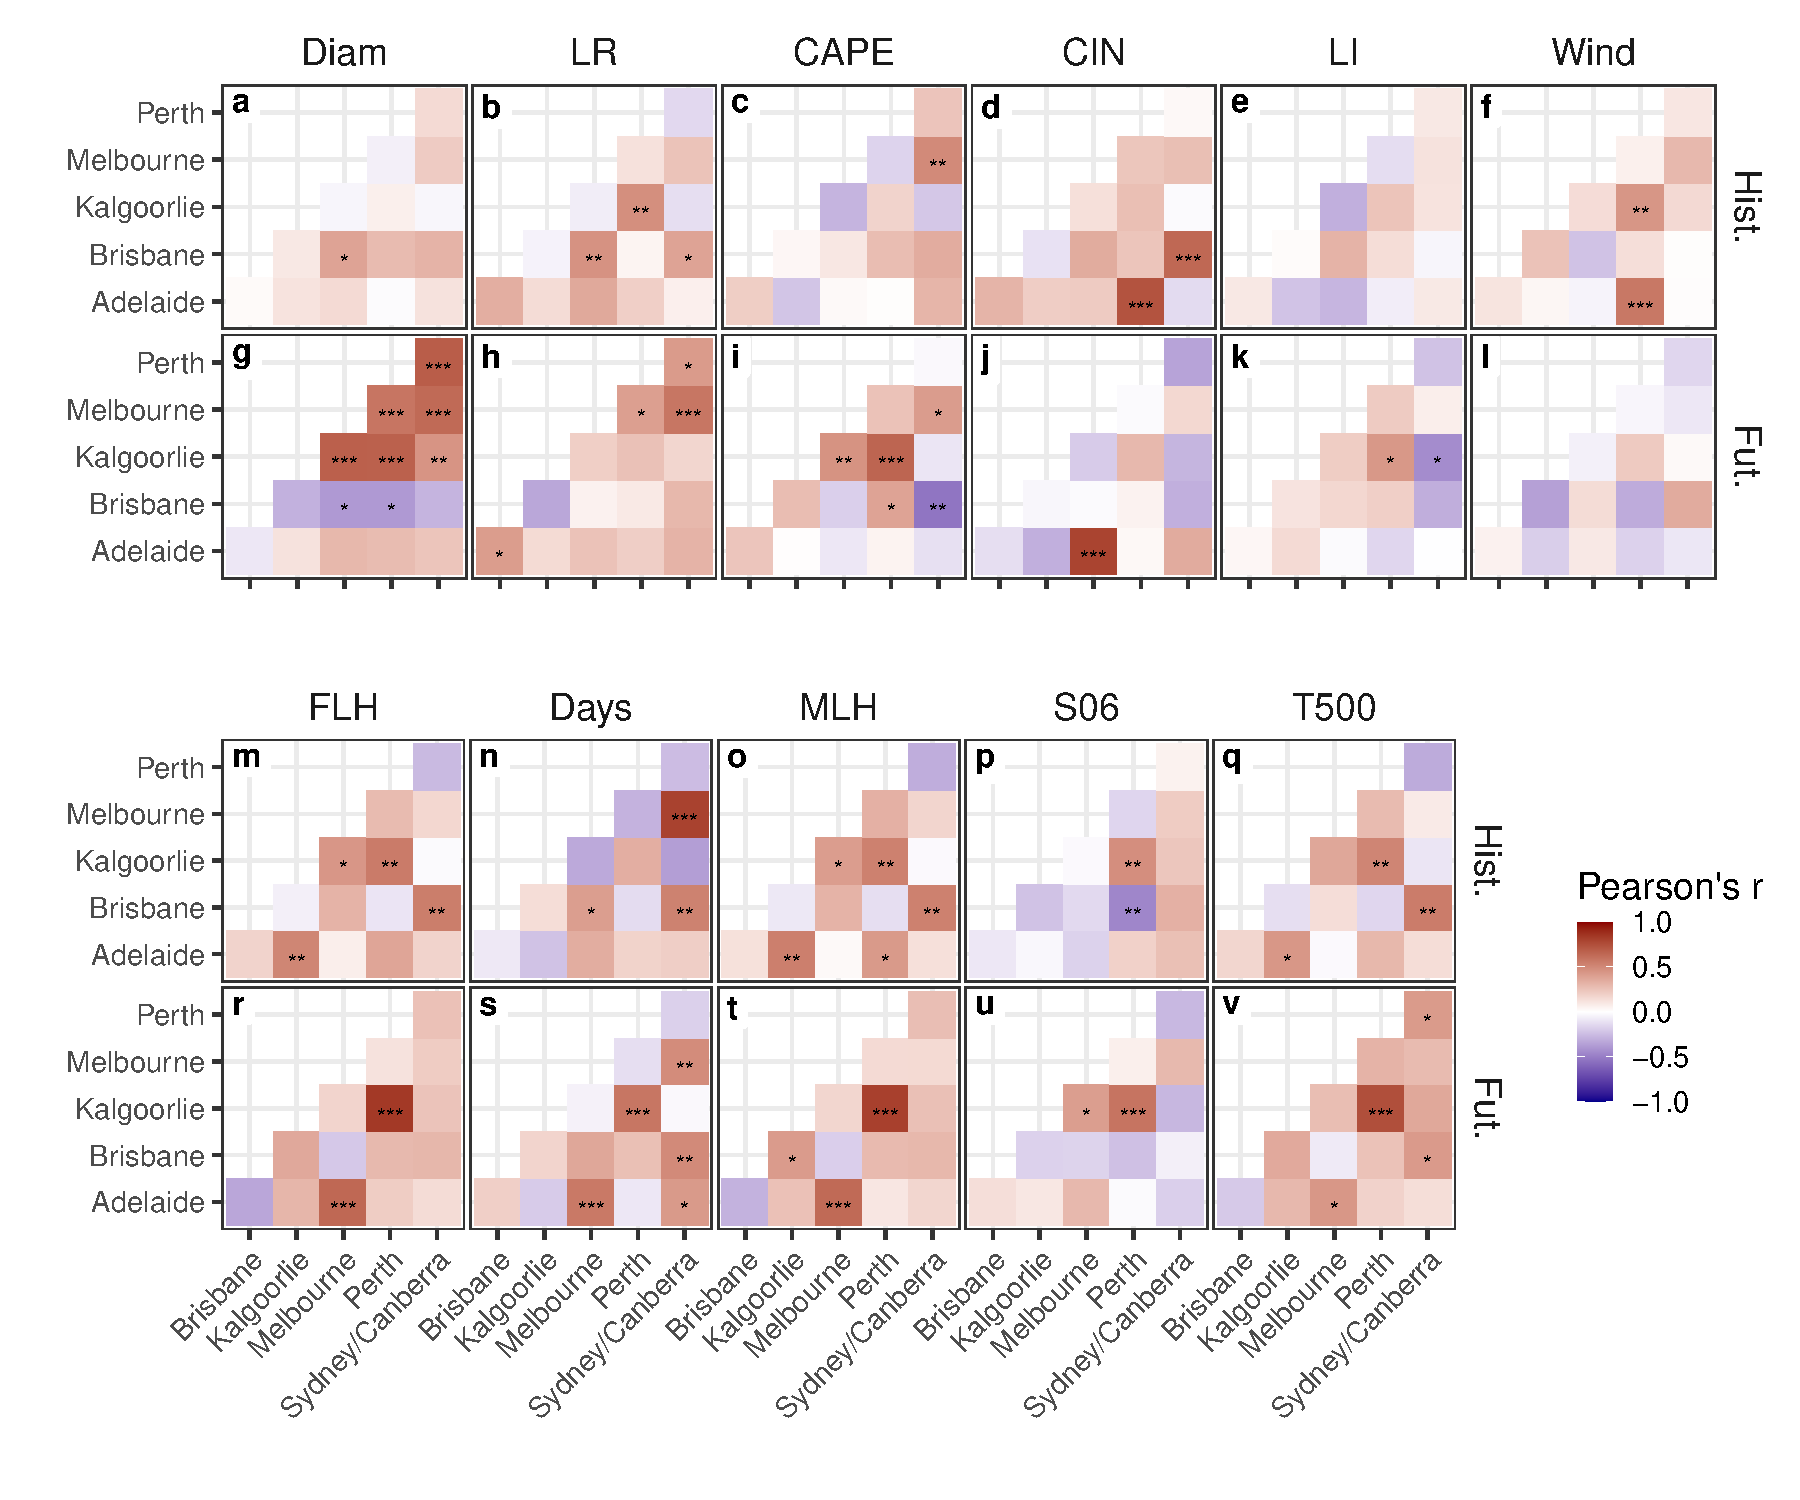
\includegraphics[width=\textwidth]{figures/correlations}
      \caption{Correlations of seasonal values of hail-relevant properties
      between domains, by epoch. Seasonal means were calculated from daily means
      at hail locations and hours. Variables considered are seasonal hail days
      (a, g), and mean hail diameter (b, h), 10 m wind at hail hours (c, i),
      bulk vertical wind shear (d, j), CAPE (e, k), lifted index (f, l), CIN (m,
      r), 700-500 hPa lapse rate (n, s), temperature at 500 hPa (o, t), freezing
      level height (p, u) and melting level height (q, v), for historical (a-f,
      m-q) and future (g-l, r-v) epochs. Statistically significant correlations
      are shown by an $\ast{}$ for 90\% confidence level ($p <$ 0.1),
      $\ast{}\!\ast{}$ for 95\% confidence level ($p <$ 0.05), and
      $\ast{}\!\ast{}\!\!\ast{}$ for the 99\% confidence level ($p <$ 0.01).}
      \label{fig:correlations}
\end{figure}

\section{Conclusions}

In this study we used downscaled regional analyses to project changes in hail
diameter and coincident wind speeds in warmer conditions, over hail-prone
regions of Australia. The climate scenario considered was for SSP2-4.5 for the
period 2080--2099 compared to a 1989--2019 baseline, using \todo{eight} CMIP
ensemble members. The domains covered more than 60\% of Australia's population,
including the major cities of Perth, Adelaide, Melbourne, Canberra, Sydney, and
Brisbane. The results show projected increases in hail frequency around
Sydney/Canberra and Brisbane, projected increases in hail size around
Sydney/Canberra and Melbourne, and indications of increased wind at hail hours
in Adelaide and the remote Goldfields region but decreased probability of
damaging wind at hail hours in Melbourne, Perth, and Sydney/Canberra. An
analysis of the changes in mean atmospheric conditions at hail hours shows
projected increases in atmospheric instability and freezing level height, and
little change in bulk vertical wind shear in the warmer scenario. Correlations
in seasonal average hail size between regions are stronger in the future than
present scenario. \todo{JA: Conclusion – add quantification}

\todo{Relate changes to similar studies, eg for wind.}

Several caveats apply to the results shown here. The most notable is that
maximum hail sizes reported at each hour are maximums over the last hour, while
wind speeds are instantaneous values within the temporal vicinity of hail
occurrence. Maximum wind gusts over the previous hour would generally be
significantly stronger than these instantaneous values. We also caution that
these results are one realization of possible future projections, based on the
boundary conditions and modelling framework used, and more ensemble members
using different setups are required to build a more complete picture of possible
future hazards.

\todo{JA: Note on storm season – 2 of our top 20 hail events occurred in Autumn
- Rockhampton hail storm April 2020 and Gosford hail May 2023 (and the 1999
Sydney hail storm occurred in April too)}

\todo{JA: future work, applicability to insurance industry and building code,
impact of correlation bt regions on insurance and building recovery. See
paragraph at end of this document. }

\todo{JA's text:} This study shows that the frequency and severity of damaging
hail events may increase in major population centres of Australia in a warming
climate. This poses an increasing risk to communities in terms of personal
safety and through building damage, solar panel damage, water ingress and damage
to interiors, contents and cars and loss of use of commercial, civil and
residential buildings for extended periods. The damage from giant hail events
can be extreme causing extensive structural damage and complete loss of amenity
of a building and widespread community disruption as seen in the 2020 Halloween
hailstorm in southeastern Queensland. The increasing correlation of hail events
in multiple cities poses a challenge to community resilience for the increased
resources required for rebuilding efforts. For insurers, storm losses account
for a quarter of all Australian natural catastrophe losses (Insurance Council of
Australia, 2024) and this is likely to increase in the future as giant hail
events increase in key centres, which may result in higher insurance premiums
and reinsurance costs.

These projections could be incorporated into the Australian building code, which
as mentioned in the Introduction does not consider hail loading, to strengthen
the resilience of buildings in the face of a changing climate. 

Future work in this area may include consideration of the win-driven hail
processes and how they may change with climate change at higher resolution,
extension to other countries such as New Zealand and extension to a wider range
of climate scenarios and timeframes.

\section*{Open Research Section}

Boundary condition data are available at \citeA{Xu_code_data_2021}. Complete
analysis code and WRF configuration files are available in a \todo{Zenodo
repository}. Convective parameters were calculated using \texttt{xarray\_parcel}
(DOI: 10.5281/zenodo.8088497).

% This section MUST contain a statement that describes where the data supporting
% the conclusions can be obtained. Data cannot be listed as ''Available from
% authors'' or stored solely in supporting information. Citations to archived
% data should be included in your reference list. Wiley will publish it as a
% separate section on the paper’s page. Examples and complete information are
% here: https://www.agu.org/Publish with AGU/Publish/Author Resources/Data for
% Authors

\acknowledgments

Since March 2024, THR's position at UNSW Sydney has been supported by QBE
Insurance. This research was undertaken with the assistance of resources from
the National Computational Infrastructure (NCI Australia), an NCRIS enabled
capability supported by the Australian Government. We thank Simon Tett for
useful discussions on extreme value techniques.

%% Include references from supporting information.
\nocite{Milbrandt_JAS_2021}
 \nocite{Zhang_JC_2017}
 \nocite{Iacono_JGRA_2008}
 \nocite{Hong_MWR_2006}
 \nocite{Jimenez_MWR_2012}
 \nocite{Niu_JGRA_2011}


\bibliography{library}

\end{document}
